% Бүлэг 1

\chapter{Онолын хэсэг} % Бүлгийн нэр
\label{Chapter1} % Энэ бүлэг рүү ишлэл хийх бол \ref{Chapter1} командыг ашигла 
\pagecolor{white}
%-------------------------------------------------------------------------------

% Агуулгад ашигласан хэвшүүлэлтийн зарим командын тодорхойлолт
\newcommand{\keyword}[1]{\textbf{#1}}
\newcommand{\tabhead}[1]{\textbf{#1}}
\newcommand{\code}[1]{\texttt{#1}}
\newcommand{\file}[1]{\texttt{\bfseries#1}}
\newcommand{\option}[1]{\texttt{\itshape#1}}

%-------------------------------------------------------------------------------

\section{Веб сайт гэж юу вэ?}
Веб сайт гэдэг нь веб сервер дээр хадгалагдаж, интернэтээр нэвтрэх боломжтой, хоорондоо холбогдсон веб хуудас эсвэл баримт бичгийн цуглуулга юм. Энэ нь ихэвчлэн өвөрмөц домэйн нэрээр тодорхойлогддог бөгөөд веб хөтчөөр дамжуулан ханддаг. Вэбсайтууд нь хэрэглэгчдэд мэдээлэл, нөөц, үйлчилгээ, үзвэр үйлчилгээ үзүүлэх зорилготой юм. Тэдгээрийг хувийн блог, онлайн дэлгүүр, мэдээллийн портал, боловсролын платформ, нийгмийн сүлжээний сайт гэх мэт янз бүрийн зорилгоор үүсгэж болно. \\
Вебсайт нь текст, зураг, видео, аудио болон интерактив элементүүдийг агуулж болох бөгөөд энэ нь хэрэглэгчдэд өөр өөр хуудсаар аялах, мэдээлэл авах, маягт илгээх, худалдан авалт хийх, контенттой харилцах боломжийг олгодог. Вебсайтууд нь байнга өөрчлөгддөггүй тогтмол агуулгатай, динамик байж болох бөгөөд энэ нь хэрэглэгчийн оролт эсвэл мэдээллийн сангийн асуулгад тулгуурлан динамикаар үүсгэгдэж, шинэчлэгддэг. Вебсайтуудыг HTML (Hypertext Markup Language), CSS (Cascading Style Sheets), JavaScript зэрэг веб технологи, PHP, Python, Ruby зэрэг сервер талын скрипт хэлүүдийг ашиглан бүтээдэг. Эдгээр технологи нь нүдэнд харагдахуйц, интерактив веб хуудас үүсгэх боломжийг олгодог. \\
Ерөнхийдөө веб сайтууд нь харилцаа холбоо, мэдээлэл солилцох, онлайн гүйлгээ хийх боломжийг бүрдүүлэхэд чухал үүрэг гүйцэтгэдэг бөгөөд хувь хүн, бизнес эрхлэгчдэд онлайн байр суурийг бий болгох, интернэтэд хэрэглэгчидтэй харилцах үндсэн хэрэгсэл болдог. Веб сайт гэдэг нь веб сервер дээр хадгалагдаж, интернэтээр нэвтрэх боломжтой, хоорондоо холбогдсон веб хуудас эсвэл баримт бичгийн цуглуулга юм. Энэ нь ихэвчлэн өвөрмөц домэйн нэрээр тодорхойлогддог бөгөөд веб хөтчөөр дамжуулан ханддаг.\\
Вeбсайтууд нь хэрэглэгчдэд мэдээлэл, нөөц, үйлчилгээ, үзвэр үйлчилгээ үзүүлэх зорилготой юм. Тэдгээрийг хувийн блог, онлайн дэлгүүр, мэдээллийн портал, боловсролын платформ, нийгмийн сүлжээний сайт гэх мэт янз бүрийн зорилгоор үүсгэж болно. Вэбсайт нь текст, зураг, видео, аудио болон интерактив элементүүдийг агуулж болох бөгөөд энэ нь хэрэглэгчдэд өөр өөр хуудсуудаар аялах, мэдээлэл авах, маягт илгээх, худалдан авалт хийх, контенттой харилцах боломжийг олгодог. Вeбсайтууд нь байнга өөрчлөгддөггүй тогтмол агуулгатай, динамик байж болох бөгөөд энэ нь хэрэглэгчийн оролт эсвэл мэдээллийн сангийн асуулгад тулгуурлан динамикаар үүсгэгдэж, шинэчлэгддэг. Вебсайтуудыг HTML (Hypertext Markup Language), CSS (Cascading Style Sheets), JavaScript зэрэг веб технологи, PHP, Python, Ruby зэрэг сервер талын скрипт хэлүүдийг ашиглан бүтээдэг. Эдгээр технологи нь нүдэнд харагдахуйц, интерактив веб хуудас үүсгэх боломжийг олгодог. Ерөнхийдөө веб сайтууд нь харилцаа холбоо, мэдээлэл солилцох, онлайн гүйлгээ хийх боломжийг бүрдүүлэхэд чухал үүрэг гүйцэтгэдэг бөгөөд хувь хүн, бизнес эрхлэгчдэд онлайн байр суурийг бий болгох, интернэтэд хэрэглэгчидтэй харилцах үндсэн хэрэгсэл болдог.\\
\textbf{Веб сайтын ажиллагаа }\\
Веб сайтын гүйцэтгэл гэдэг нь веб сайт хэр хурдан бөгөөд үр дүнтэй ачаалагдаж, хэрэглэгчийн харилцан үйлчлэлд хариу үйлдэл үзүүлэхийг хэлнэ. Энэ нь хэрэглэгчийн эерэг туршлагыг бий болгох, зочдыг татах, мэдээллээр хангах, гүйлгээг хөнгөвчлөх зэрэг веб сайтын зорилгод хүрэх чухал хүчин зүйл юм. Веб сайтын гүйцэтгэлд хэд хэдэн гол хүчин зүйл нөлөөлдөг: 
\begin{itemize}
    \item [1.] \textbf{Хуудас ачаалах хугацаа:}
\end{itemize}
Энэ нь веб хуудас хэрэглэгчийн хөтөч дээр хэр хурдан бүрэн ачаалагдахыг хэлнэ. Ачаалах хугацаа илүү хурдан байх нь хэрэглэгчийн сэтгэл ханамжийг сайжруулж, үсрэх хурдыг бууруулдаг. Серверийн хариу өгөх хугацаа, файлын хэмжээ, кэш хийх механизм, код болон скриптүүдийн үр ашиг зэрэг хуудас ачаалах хугацаанд янз бүрийн хүчин зүйл нөлөөлдөг. 2. Хариуцлагатай байдал: Хариуцлагатай веб сайт нь дэлгэцийн янз бүрийн хэмжээ, төхөөрөмжид тохируулан зохион байгуулалт, агуулгыг нь тохируулж, ширээний компьютер, зөөврийн компьютер, таблет, ухаалаг гар утсан дээр хэрэглэгчийн оновчтой туршлагыг хангадаг. Хариуцлагатай загвар нь хүртээмжтэй байдал, хэрэглэгчийн оролцоонд маш чухал юм.
\begin{itemize}
    \item [2.] \textbf{Серверийн гүйцэтгэл:}
\end{itemize}
Вэбсайтыг байршуулах веб серверийн гүйцэтгэл нь түүний хурд, хүртээмжид ихээхэн нөлөөлдөг. Серверийн нөөц, тохиргоо, серверийн программ хангамжийн үр ашиг, сүлжээний холболт зэрэг хүчин зүйлүүд нь вэбсайтын гүйцэтгэлд чухал үүрэг гүйцэтгэдэг. 4. Сүлжээний хоцрогдол: Хэрэглэгчийн төхөөрөмж болон веб сервер хооронд өгөгдөл дамжуулахад шаардагдах хугацаа нь вэбсайтын гүйцэтгэлд нөлөөлдөг. Хэрэглэгчийн интернэт холболтын хурд, газарзүйн байршил, сүлжээний ачаалал зэрэг хүчин зүйлүүд нь хоцролтод нөлөөлдөг. 
\begin{itemize}
    \item [3.] \textbf{Оновчтой контент:}
\end{itemize}
Зураг, скрипт, загварын хуудас зэрэг вэбсайтын агуулгыг оновчтой болгох нь файлын хэмжээг багасгаж, ачаалах хугацааг сайжруулахад тусалдаг. Шахах, багасгах, залхуу ачаалах гэх мэт техникүүд нь дамжуулах шаардлагатай өгөгдлийн хэмжээг багасгаснаар гүйцэтгэлийг сайжруулдаг.
\begin{itemize}
    \item [4.] \textbf{Browser Rendering:}
\end{itemize}
Янз бүрийн веб хөтчүүд веб сайтыг өөр өөрөөр үзүүлж, гүйцэтгэлд нөлөөлж болно. Хэрэглэгчийн тогтвортой туршлагыг хангахын тулд алдартай хөтөч дээр вэбсайтын гүйцэтгэлийг туршиж, оновчтой болгох нь чухал юм. 
\begin{itemize}
    \item [5.] \textbf{Кэш хийх:}
\end{itemize}
Кэш нь хэрэглэгчийн төхөөрөмж эсвэл завсрын серверүүд дээр байнга ханддаг веб сайтын элементүүдийг (зураг, загварын хуудас, JavaScript файлууд гэх мэт) хадгалах явдал юм. Кэш хийх нь эдгээр нөөцийг дахин дахин татах хэрэгцээг багасгаж, ачаалах хугацааг сайжруулж, серверийн ачааллыг бууруулдаг. Ачаалах хугацаа, хуудасны хэмжээ, хэрэглэгчийн зан төлөв зэрэг веб сайтын гүйцэтгэлийн хэмжигдэхүүнийг хянаж, дүн шинжилгээ хийх нь гүйцэтгэлийн саад тотгор, сайжруулах шаардлагатай газруудыг тодорхойлоход тусална. Гүйцэтгэлийг оновчтой болгох арга техникийг хэрэгжүүлэх, контент түгээх сүлжээг (CDN) ашиглах, веб сайтын дэд бүтцийг тогтмол засварлаж, шинэчлэх нь вэбсайтыг хурдан бөгөөд найдвартай болгоход хувь нэмрээ оруулж чадна.\\
Веб сайт хэрхэн ажилладаг вэ?
\begin{figure}[ht]
    \centering
    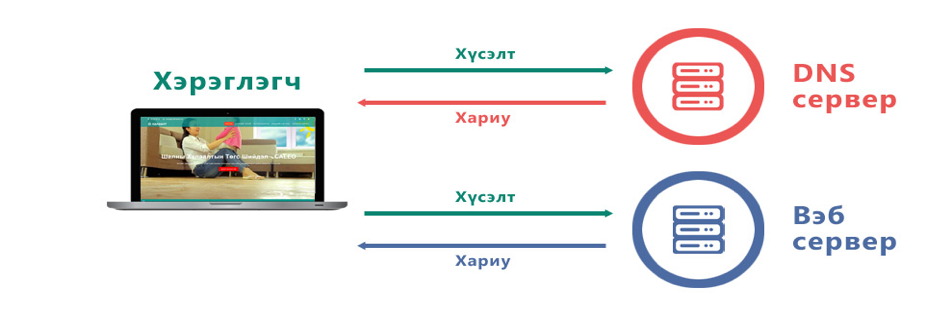
\includegraphics[scale=0.8]{Figures/pic11.png}
    \caption{Вэб сайтын ажиллагаа}
    \label{fig11}
\end{figure}\\
\newpage
Вэб сайтын ажиллагааг мэдэхийн тулд хэрэглэгч болон сервер (client, server) хоёрын хооронд явагддаг хүсэлт-хариулт (request-response), домэйн нэрийн систем буюу DNS гэсэн ойлголт хэрэгтэй.\\
\textbf{HTTP хүсэлт-хариултын загвар}\\
Хэрэглэгч компьютер эсвэл гар утасныхаа вэб хөтөч програмын хаягийн мөрөнд (address bar) орж үзэх гэж байгаа сайтынхаа url хаягийг бичээд Enter товч дарахад тухайн сайтын байрлаж буй сервер лүү HTTP хүсэлт илгээгдэнэ. Серверт суулгасан тусгай вэб-сервер програм нь (Apache, IIS, Nginx) хүсэлтийг амжилттай хүлээн авсан тохиолдолд шаардлагатай мэдээллийг агшин зуур боловсруулаад HTTP хариу болгон хэрэглэгчийн компьютер луу илгээнэ. Амжилтгүй бол алдааны код илгээдэг.\\
\textbf{Статик сайтын хувьд:}
\begin{itemize}
    \item [•] Серверийн хариу нь хэрэглэгчийн хүссэн тодорхой HTML хуудас байдаг.
    \item [•] HTML хуудаснууд нь физик буюу бодит байна.
    \item [•] Хэрэглэгч сайтын нүүр хуудас руу хандсан бол index.html эсвэл index.htm файлууд дуудагддаг.
\end{itemize}
\textbf{Динамик сайтын хувьд:}
\begin{itemize}
    \item [•] Сервер нь хэрэглэгчийн хүсэлтийг цааш нь PHP хөрвүүлэгч рүү дамжуулна. PHP хөрвүүлэгч ирсэн хүсэлтийг боловсруулсны дараа хөрвүүлсэн кодыг сервер нь хариу болгон хэрэглэгч рүү HTML тэмдэглэгээ хэлбэрээр илгээдэг.
    \item [•] Хуудаснууд нь байнга скрипт хэлээр боловсруулагдан үүсгэгддэг.
    \item [•] Сайтын нүүр хуудас руу хандахад index.php файл дуудагдана.
\end{itemize}
Компьютер дээрх веб хөтөч программ (Google Chrome, Firefox, Interner Explorer, Opera г.м.) нь серверээс ирсэн хариуг боловсруулаад тухайн веб хуудасны мэдээлэл буюу текст, зураг, видео зэргийг хэрэглэгчид тохиромжтой хэлбэрээр дэлгэцэнд харуулдаг. Хуудасны мэдээлэл нь HTML тэмдэглэгээт хэлээр үүсгэгдсэн байна. Хэрэв та Chrome, Firefox ашигладаг бол Ctrl + U товчийг дарж хуудасны эх кодыг үзэж болно.\\
Энгийнээр бол веб сайтын ажиллагаа гэдэг нь интернэтэд холбогдсон хоёр компьютерын (хэрэглэгчийн компьютер буюу client, веб сайт байрлаж байгаа супер компьютер буюу server) хооронд HTTP протоколоор явагддаг мэдээллийн солилцоо гэж ойлгож болно. Нэг супер компьютер дээр хоорондоо уялдаатай эсвэл тусдаа ажиллагаатай хэдэн ч веб-сервер программ суулгасан байж болно. Харин нэг вэб-сервер дээр хэдэн ч вэбсайт байрлаж болно (тухайн сервер-компьютерын санах ойноос хамаардаг).\\
\textbf{Веб хөтөч программ нь DNS серверийн IP хаягийг хэрхэн олдог вэ? }\\
Хэрэглэгчийн гэрийн эсвэл ажлын интернэтийн холболтын төхөөрөмжид DNS тохиргоо хийгдсэн байдаг. Интернэтийн үйлчилгээ үзүүлдэг компаний ажилтан интернэтэд холбохдоо DNS тохиргоог хийдэг. Домэйн нэрийн системийн серверүүд нэгдсэн зарчмаар ажилладаг.
\section{HTML хэл}
HTML нь HyperText Markup Language гэсэн үгийн товчлол юм. Энэ нь тэмдэглэгээний хэлийг ашиглан вeб хуудасны дизайн хийхэд хэрэглэгддэг. HTML нь Hypertext болон Markup хэлний хослол юм. Гипертекст нь вeб хуудсуудын хоорондын холбоосыг, тэмдэглэгээний хэл нь вeб хуудасны бүтцийг тодорхойлдог шошгон доторх текст баримт бичгийг тодорхойлдог.\\
\textbf{HTML юунд ашиглагддаг вэ? }\\
HTML нь World Wide Web (www) дээр харагдах вэб хуудасны бүтцийг бий болгоход хэрэглэгддэг. Энэ нь вeб хуудасны дизайн хийхэд ашигладаг шошго ба шинж чанаруудыг агуулдаг. Мөн бид Hyperlink ашиглан олон хуудсыг холбох боломжтой.\\
\textbf{HTML үндсэн форматын хуудасны бүтэц}\\
HTML хуудасны үндсэн бүтцийг доор харуулав. Энэ нь бүх вэб хуудсыг үүсгэх үндсэн элементүүдийг (жишээлбэл, баримт бичгийн төрөл, HTML, толгой, гарчиг, биеийн элементүүд) агуулдаг.
\begin{figure}
    \centering
    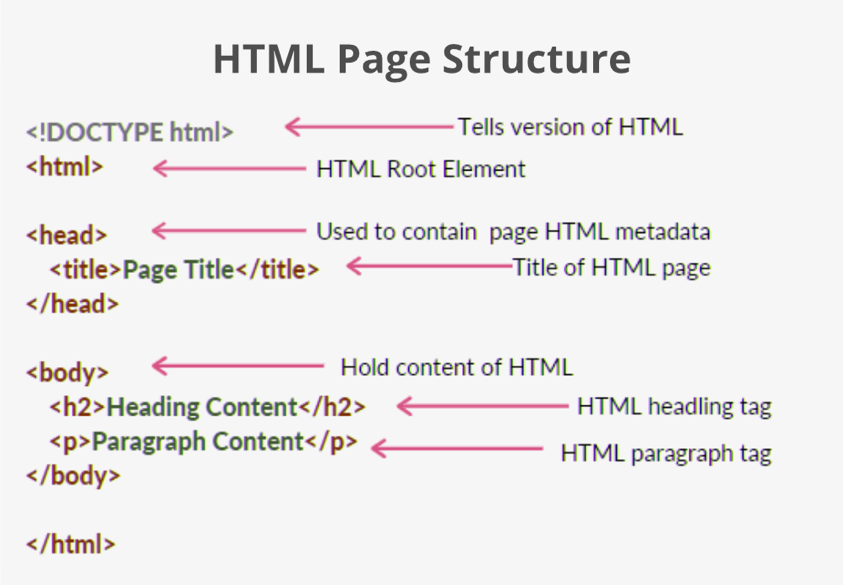
\includegraphics[scale=0.8]{Figures/pic12.png}
    \caption{HTML хэлний бүтэц}
    \label{fig12}
\end{figure}
\begin{itemize}
    \item [•] \textbf{<DOCTYPE! html>} – Баримт бичгийн төрөл эсвэл баримт бичгийн төрлийн мэдэгдэл нь веб хөтчид одоогийн хуудас бичигдсэн тэмдэглэгээний хэлийг хэлдэг заавар юм. Энэ нь элемент эсвэл шошго биш юм. Баримт бичгийн хэв маягийн мэдэгдэл нь том жижиг жижиг үсгийг харгалздаггүй.
    \item [•] \textbf{<html>} – Энэ таг нь HTML баримтын үндсэн элементийг тодорхойлоход хэрэглэгддэг. Энэ шошго нь хөтчид HTML баримт бичиг гэдгийг хэлдэг. Энэ нь бусад бүх элементүүдийг агуулсан хоёр дахь гаднах савны элемент юм.
    \item [•] \textbf{<head>} – Энэ таг нь баримт бичигтэй холбоотой мэдээллийг агуулсан HTML баримтын толгой хэсгийг тодорхойлоход хэрэглэгддэг. Толгойн шошго доторх элементүүд веб хуудасны нүүрэн талд харагдахгүй байна.
    \item [•] \textbf{<body>} – Биеийн таг нь вэб хуудасны харагдах бүх агуулгыг хаахад хэрэглэгддэг. Өөрөөр хэлбэл, үндсэн контент нь хөтөчийн нүүрэн талд харуулах зүйл юм.
\end{itemize}
\section{CSS гэж юу вэ?}
CSS нь Cascading Style Sheets гэсэн үгийн товчлол юм. Энэ нь HTML (Hypertext Markup Language) дээр бичигдсэн баримт бичгийн харагдах байдал, форматыг тодорхойлоход хэрэглэгддэг загварын хуудасны хэл юм. CSS нь веб хөгжүүлэгчдэд веб хуудсуудын бүтэц, өнгө, фонт, хөдөлгөөнт дүрс гэх мэт харагдах байдлыг хянах боломжийг олгодог. Энэ нь веб хуудасны танилцуулгыг агуулгаас нь салгах арга замыг бий болгож, вебсайтын дизайныг хадгалах, шинэчлэхэд хялбар болгодог.\\
\textbf{Синтакс}\\
CSS нь энгийн синтакстай бөгөөд янз бүрийн загварын шинж чанаруудын нэрийг зааж өгөхийн тулд хэд хэдэн англи түлхүүр үгсийг ашигладаг.\\
Загварын хуудас нь дүрмийн жагсаалтаас бүрдэнэ. Дүрэм эсвэл дүрмийн багц бүр нь нэг буюу хэд хэдэн сонгогч, мэдэгдлийн блокоос бүрдэнэ.\\
\textbf{CSS-ийн зарим ерөнхий ойлголт, зарчмуудыг энд оруулав.}
\begin{itemize}
    \item [1.] \textbf{Сонгогчид:} CSS нь тодорхой HTML элементүүдийг чиглүүлэх, тэдгээрт хэв маяг хэрэглэхийн тулд сонгогчийг ашигладаг. Сонгогчид нь элементийн нэр, анги, ID, шинж чанар эсвэл шаталсан харилцаанд тулгуурлаж болно.
    \item [2.] \textbf{Properties ба утгууд:} CSS шинж чанарууд нь өнгө, фонт, хэмжээ, зах, дэвсгэр, хүрээ гэх мэт элементийн харагдах байдлын тодорхой талыг тодорхойлдог. Үл хөдлөх хөрөнгө тус бүрт өөрийн онцлог шинж чанарыг тодорхойлдог утгыг өгдөг.
    \item [3.] \textbf{Хайрцагны загвар:} Хайрцагны загвар нь элементүүдийг тэгш өнцөгт хайрцаг хэлбэрээр хэрхэн харуулахыг тайлбарладаг. Энэ нь агуулга, дэвсгэр, хүрээ, захаас бүрдэнэ. Эдгээр шинж чанарууд нь элементүүдийн хэмжээ, зай, байршлыг хянадаг.
    \item [4.] \textbf{Каскад ба өвөрмөц байдал:} CSS-ийн "cascading" гэсэн нэр томъёо нь тэдгээрийн өвөрмөц байдал, харагдах дарааллаар нь элементүүдэд хэв маягийг хэрэглэх арга замыг хэлнэ. Элементтэй ойртож тодорхойлсон загварууд нь холоос тодорхойлсон загваруудаас давуу эрхтэй болно.
    \item [5.] \textbf{Responsive дизайн:} CSS нь хариу үйлдэл үзүүлэх веб дизайныг идэвхжүүлдэг бөгөөд энэ нь веб хуудсуудыг өөр өөр төхөөрөмж, дэлгэцийн хэмжээтэй тааруулж, хариу үйлдэл үзүүлэх боломжийг олгодог. Хэвлэл мэдээллийн асуулга нь үзэх орчны онцлогт тулгуурлан өөр өөр хэв маягийг хэрэглэхэд ашиглагддаг.
    \item [6.] \textbf{Layout and Positioning:} CSS нь веб хуудасны элементүүдийн байршил, байршлыг хянах янз бүрийн арга техникээр хангадаг. Үүнд float, flexbox, grid зэрэг техник, харьцангуй, үнэмлэхүй, тогтмол гэх мэт байрлал тогтоох шинж чанарууд орно.
    \item [7.] \textbf{Загварын шатлал:} CSS нь эх элементүүдээс хүүхэд элементүүд рүү хэв маягийг өвлүүлэх боломжийг олгодог. Энэ нь дэлхийн хэмжээнд хэв маягийг тодорхойлж, тэдгээрийг үүрлэсэн элементүүдэд ашиглах боломжтой болгодог.
    \item [8.] \textbf{CSS Preprocessors:} Sass болон Less гэх мэт CSS-ийн урьдчилсан боловсруулагч нь хувьсагч, холимог, функц, үүрлэсэн синтакс зэрэг нэмэлт функцуудыг нэвтрүүлдэг. Эдгээр урьдчилсан процессорууд нь CSS кодын бүтээмж, тогтвортой байдлыг сайжруулдаг.
\end{itemize}
CSS-ийг ашигласнаар веб хөгжүүлэгчид нүдэнд харагдахуйц, дизайн үүсгэж, хэрэглэгчийн туршлагыг сайжруулж, өөр өөр веб хөтөч болон төхөөрөмжүүдийн нийцтэй байдлыг хангах боломжтой. Энэ нь HTML элементүүдийн танилцуулгыг өөрчлөх, дизайны тодорхой шаардлагад нийцүүлэн тохируулах уян хатан байдлыг хангадаг.
\section{JavaScript гэж юу вэ?}
JavaScript бол динамик, интерактив веб хуудас үүсгэхэд өргөн хэрэглэгддэг өндөр түвшний программчлалын хэл юм. Энэ нь үндсэндээ үйлчлүүлэгч тал дээр хийгддэг бөгөөд энэ нь хэрэглэгчийн веб хөтөч дээр ажилладаг гэсэн үг юм. JavaScript нь хөгжүүлэгчдэд веб хуудсанд функц нэмэх, контентыг удирдах, өөрчлөх, хэрэглэгчийн үйлдэлд хариу үйлдэл үзүүлэх, серверүүдтэй харилцах боломжийг олгодог. Энэ нь объект хандалтат, императив, функциональ программчлалын парадигмуудыг дэмждэг олон талт хэл юм.
\begin{figure}[ht]
    \centering
    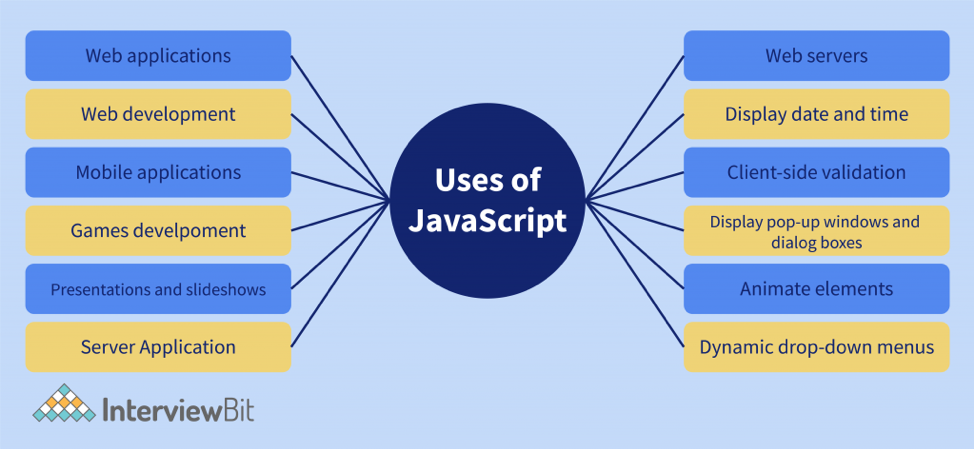
\includegraphics[scale=0.8]{Figures/pic13.png}
    \caption{JavaScript-ийн хэрэглээ}
    \label{fig13}
\end{figure}
\textbf{JavaScript-н зарим нийтлэг хэрэглээ:}
\begin{itemize}
    \item [1.] Веб хөгжүүлэлт: JavaScript нь веб хөгжүүлэлтэд голчлон ашиглагддаг. Энэ нь веб хуудасны интерактив болон динамик элементүүдийг идэвхжүүлдэг, тухайлбал маягтыг баталгаажуулах, DOM удирдах (веб хуудасны агуулга, бүтцийг өөрчлөх), үйл явдлуудыг зохицуулах (товчлуур товших, хулганы хөдөлгөөн гэх мэт), серверт асинхрон хүсэлт гаргах (AJAX). 
    \item [2.] Front-end Development: JavaScript нь урд талын программыг хөгжүүлэхэд зайлшгүй шаардлагатай. Энэ нь интерактив хэрэглэгчийн интерфейс үүсгэх, үйлчлүүлэгчийн баталгаажуулалтыг хэрэгжүүлэх, төлөвийг удирдах, хэрэглэгчийн харилцан үйлчлэлийг зохицуулах, API болон гуравдагч талын номын сангуудтай нэгтгэхэд HTML болон CSS-тэй хамт хэрэглэгддэг. 
    \item [3.] Single-Page Applications (SPAs): React, Angular, Vue.js зэрэг JavaScript фреймворкуудыг SPA-г бүтээхэд өргөн ашигладаг. Эдгээр хүрээ нь бүрэлдэхүүн хэсгүүдийг үр дүнтэй гаргах, программын төлөвийг удирдах, хэрэглэгчийн туршлагыг жигд, хариу үйлдэл үзүүлэх боломжийг олгодог. 4. Гар утасны программ хөгжүүлэлт: React Native болон Ionic зэрэг JavaScript хүрээ нь хөгжүүлэгчдэд JavaScript ашиглан гар утасны программ бүтээх боломжийг олгодог. Эдгээр хүрээ нь нэг кодын бааз бүхий платформ хоорондын гар утасны программуудыг хөгжүүлэх боломжийг олгодог. 
    \item [4.] Сервер талын хөгжүүлэлт: Node.js гарч ирснээр JavaScript-г сервер талын хөгжүүлэлтэд ашиглаж болно. Node.js нь сервер дээр JavaScript-г ажиллуулах боломжийг олгодог ажиллах орчинг бүрдүүлдэг. Энэ нь өргөтгөх боломжтой, өндөр гүйцэтгэлтэй веб сервер, API болон бодит цагийн программуудыг бүтээх боломжийг олгодог. 6. Тоглоом хөгжүүлэлт: JavaScript нь HTML5 canvas болон WebGL-ийн хамт хөтөч дээр суурилсан тоглоом, интерактив график үүсгэхэд ашиглагдаж болно. Phaser болон Three.js зэрэг хүрээнүүд нь JavaScript ашиглан тоглоом хөгжүүлэх хүчирхэг хэрэгслээр хангадаг. 
    \item [5.] Өгөгдлийн дүрслэл: D3.js, Chart.js, Highcharts зэрэг JavaScript сангууд нь веб хуудсан дээр динамик, интерактив өгөгдлийн дүрслэл үүсгэх боломжийг хөгжүүлэгчдэд олгодог. Эдгээр сангууд нь өргөн хүрээний диаграм, график, дүрслэх хэрэгслүүдээр хангадаг. 8. Ширээний программууд: Electron зэрэг JavaScript фреймворкууд нь веб технологи ашиглан платформ хоорондын ширээний программуудыг хөгжүүлэх боломжийг олгодог. Энэ нь хөгжүүлэгчдэд танил веб хөгжүүлэлтийн хэрэгслүүд болон фреймворк ашиглан ширээний программ бүтээх боломжийг олгодог.
    \item [6.] Internet of Things (IoT): JavaScript нь Johnny-Five, Node-RED зэрэг платформуудын хамт IoT төхөөрөмжүүдийг программчлах, удирдахад ашиглагдаж болно. Энэ нь хөгжүүлэгчдэд мэдрэгчтэй харилцах, өгөгдөл цуглуулах, JavaScript ашиглан IoT төхөөрөмжийг удирдах боломжийг олгодог. JavaScript-ийн олон талт байдал, номын сан, фреймворкуудын том экосистем, янз бүрийн орчинд ажиллах чадвар нь түүнийг өөр өөр домэйн дэх өргөн хүрээний программуудад түгээмэл сонголт болгодог. 
\end{itemize}
\section{React програмчлалын хэл}
React бол хэрэглэгчийн интерфейс бүтээхэд зориулагдсан түгээмэл JavaScript номын сан юм. Энэ нь ихэвчлэн динамик, интерактив веб программуудыг бий болгоход ашиглагддаг. React нь хэрэглэгчийн интерфейс нь дахин ашиглах боломжтой, бие даасан бүрэлдэхүүн хэсгүүдэд хуваагддаг бүрэлдэхүүн хэсэг дээр суурилсан архитектурыг дагаж мөрддөг. Бүрэлдэхүүн хэсэг бүр өөрийн төлөвийг удирдаж, зөвхөн шаардлагатай өөрчлөлтүүдийг хийснээр хэрэглэгчийн интерфейсийг үр дүнтэй шинэчилдэг. \\
React нь үр дүнтэй дүрслэхийн тулд виртуал DOM (Баримт бичгийн объектын загвар) ашигладаг. Энэ нь хөгжүүлэгчдэд HTML-тэй төстэй код болон JavaScript логикийг хослуулах боломжийг олгодог JavaScript-н синтакс өргөтгөл болох JSX ашиглан код бичих боломжийг олгодог. React нь UI-г бий болгоход тунхаглалын хандлагыг хангадаг бөгөөд UI-ийн нарийн төвөгтэй харилцан үйлчлэл, шинэчлэлтүүдийг удирдахад хялбар болгодог.\\
React нь ихэвчлэн төрийн удирдлагад зориулсан Redux эсвэл нэг хуудастай программуудад чиглүүлэлт хийхэд зориулагдсан React Router зэрэг бусад номын сан эсвэл фреймворкуудтай хамт хэрэглэгддэг. Энэ нь өргөн хүрээний нөөц, гуравдагч этгээдийн номын сангуудтай, өргөн хүрээтэй, идэвхтэй нийгэмлэгтэй тул веб хөгжүүлэхэд түгээмэл сонголт болгодог.\\
\begin{figure}
    \centering
    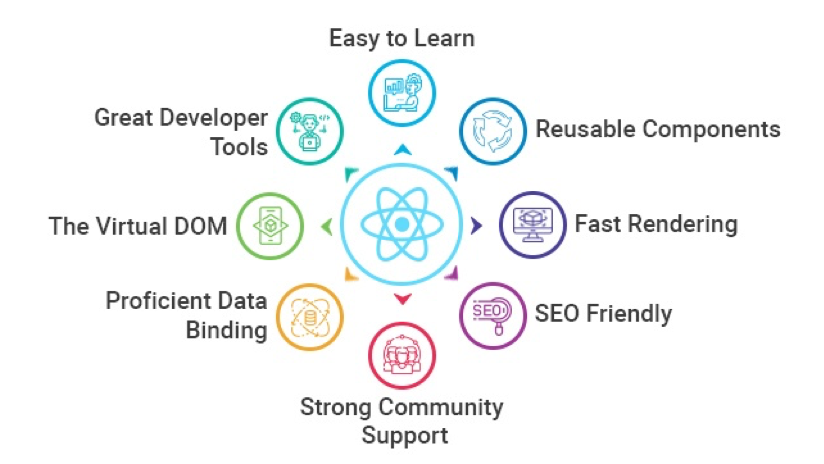
\includegraphics[scale=0.8]{Figures/pic14.png}
    \caption{Яагаад ReactJS-ийг ашиглах ёстой вэ?}
    \label{fig14}
\end{figure}\\
React нь веб программуудад хэрэглэгчийн интерфейс (UI) бүтээхэд өргөн хэрэглэгддэг JavaScript номын сан юм. Энэ нь хөгжүүлэгчдэд дахин ашиглах боломжтой UI бүрэлдэхүүн хэсгүүдийг үүсгэж, программын төлөвийг үр дүнтэй удирдах боломжийг олгодог. React-ийг хэрхэн ашиглаж болох жишээ энд байна:
\begin{itemize}
    \item [1.] React-ийг тохируулах: Эхлээд та React хөгжүүлэлтийн орчинг тохируулах хэрэгтэй. Үүнд ихэвчлэн Node.js суулгаж, npm (Node Package Manager) ашиглан шинэ React төсөл үүсгэнэ. 
    \item [2.] Бүрэлдэхүүн хэсгүүдийг үүсгэх: React программ дээр та бүрэлдэхүүн хэсгүүдийг ашиглан өөрийн UI-г бүтээдэг. Бүрэлдэхүүн хэсгүүд нь бие даасан, дахин ашиглах боломжтой UI хэсгүүд бөгөөд цогц UI бүтцийг бий болгохын тулд нэгтгэж болно. Бүрэлдэхүүн хэсгүүд нь функциональ эсвэл ангид суурилсан байж болно.
    \item [3.] Төлөвийг удирдах: React нь бүрэлдэхүүн хэсгийн өгөгдөл болон төлөвийг удирдах "төлөв" хэмээх ойлголтыг өгдөг. Төлөв нь цаг хугацааны явцад өөрчлөгдөж болох бүрэлдэхүүн хэсгийн динамик хэсгийг илэрхийлдэг. Та `setState()` аргыг ашиглан төлөвийг шинэчилж, бүрэлдэхүүн хэсгийг дахин дүрслэх боломжтой.
    \item [4.] JSX Синтакс: React нь JSX (JavaScript XML) синтаксийг ашигладаг бөгөөд энэ нь танд JavaScript файлууддаа HTML шиг код бичих боломжийг олгодог. JSX нь өөрийн бүрэлдэхүүн хэсгүүдийн бүтэц, гадаад төрхийг тодорхойлох товч бөгөөд уншихад хялбар арга юм.
    \item [5.] Бүрэлдэхүүн хэсгийн ашиглалтын мөчлөг: Урвалын бүрэлдэхүүн хэсгүүд нь бүрэлдэхүүнийг үүсгэх, шинэчлэх, устгах зэрэг өөр өөр үе шатанд дуудагддаг амьдралын мөчлөгийн аргуудтай. Эдгээр амьдралын мөчлөгийн аргууд нь бүрэлдэхүүн хэсгийн амьдралын мөчлөгийн тодорхой цэгүүдэд үйлдэл хийх боломжийг олгодог.
    \item [6.] Бүрэлдэхүүн хэсгүүдийг дүрслэх: React-ийн бүрэлдэхүүн хэсгүүдийг үзүүлэхийн тулд та `ReactDOM.render()` аргыг ашигладаг бөгөөд энэ нь үндсэн бүрэлдэхүүн хэсэг болон бүрэлдэхүүнийг үзүүлэх ёстой DOM элементийг авдаг.
    \item [7.] Үйл явдлыг зохицуулах: React нь товчлуур дарах, маягт илгээх, гарнаас оруулах зэрэг үйл явдлуудыг зохицуулах синтетик үйл явдлын системийг хангадаг. Үйл явдал зохицуулагчийг хэрэглэгчийн харилцааг зохицуулахын тулд бүрэлдэхүүн хэсгүүдэд хавсаргаж болно.
    \item [8.] Бүрэлдэхүүн хэсгүүдийг дахин ашиглах боломж: React нь бүрэлдэхүүн хэсгүүдийг дахин ашиглах боломжийг дэмжиж, модульчлагдсан, засвар үйлчилгээ хийх боломжтой код үүсгэх боломжийг танд олгоно. Бүрэлдэхүүн хэсгүүдийг бүрдүүлж, үүрлэж болох бөгөөд энэ нь шаталсан бүтэц, санаа зовоосон асуудлуудыг салгах боломжийг олгодог.
    \item [9.] Virtual DOM: React нь үр дүнтэй дүрслэхийн тулд виртуал DOM (Баримт бичгийн объектын загвар) ашигладаг. Виртуал DOM нь бодит DOM-ийн хөнгөн дүрслэл бөгөөд React нь төлөв өөрчлөгдөх үед зөвхөн UI-ийн шаардлагатай хэсгүүдийг үр дүнтэй шинэчлэхэд ашигладаг.
\end{itemize}
React нь веб хөгжүүлэлтэд өргөн хэрэглэгддэг бөгөөд түүний алдартай нь түүний бүрэлдэхүүн хэсэг дээр суурилсан архитектур, тунхаглалын синтакс, үр дүнтэй дүрслэх арга барилаас үүдэлтэй. Энэ нь түүний чадавхыг улам сайжруулж, нарийн төвөгтэй, интерактив хэрэглэгчийн интерфейсийг бүтээхэд хялбар болгодог асар том номын сан, хэрэгслүүдийн эко системтэй.\\

\textbf{Мэдээллийн томоохон байууллагууд яагаад React сонгодог вэ?}
\begin{itemize}
    \item [\textbf{1.}] \textbf{Facebook}
\end{itemize}
Facebook ReactJS-ийг ашиглаж байна. Тэдний вэб хуудас нь програмын кодонд холилдсон скрипт болох React-ээр бүтээгдсэн. Энэхүү гар утасны програм нь React Native нэртэй React-ийн хувилбараар бүтээгдсэн бөгөөд DOM элементийн оронд iOS болон Android-ийн үндсэн бүрэлдэхүүн хэсгүүдийг харуулах үүрэгтэй.
\begin{itemize}
    \item [\textbf{2.}] \textbf{Instagram}
\end{itemize}
Instagram доторх ReactJS хэрэглээ асар их. Үүний нотолгоо бол газарзүйн байршил, Google Maps API, хайлтын системийн нарийвчлал, мөн hashtagгүйгээр гарч ирдэг шошго зэрэг олон боломжууд юм. IT бүгд програмын API-д байдаг бөгөөд үнэхээр гайхалтай юм. Instagram нь бүхэлдээ ReactJS номын сан дээр суурилсан бөгөөд түүний онцлогт бүрэн дасан зохицох боломжийг олгосон.
\begin{figure}[h]
    \centering
    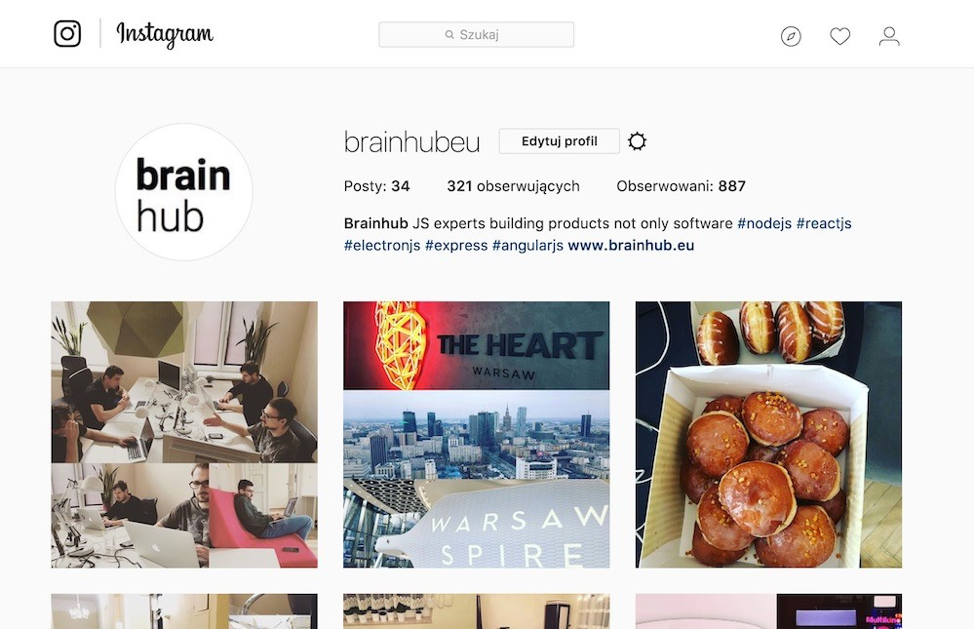
\includegraphics[scale=0.8]{Figures/pic15.png}
    \caption{Instagram хуудас}
    \label{fig15}
\end{figure}\\
\begin{itemize}
    \item [\textbf{3.}] \textbf{Netflix}
\end{itemize}
React хувилбар нь Netflix-тэй, ялангуяа вэб хөтчүүдэд ашигладаг DOM-ийн оронд бага гүйцэтгэлтэй ТВ төхөөрөмжүүдэд ашиглагддаг Gibbon нэртэй платформ дээр ажилладаг. Netflix нь ReactJS номын сан нь эхлүүлэх хурд, ажиллах цагийн гүйцэтгэл, модульчлагдсан байдал болон бусад олон давуу талуудад хэрхэн тусалдаг талаар тайлбарласан албан ёсны блог нийтлэлийг нийтэлсэн.
\begin{itemize}
    \item [\textbf{4.}] \textbf{Нью Йорк Таймс}
\end{itemize}
Хэдхэн сарын өмнө Нью Йорк Таймс сонин Оскарын улаан хивсэн дээрх оддын дүр төрхийг дуурайлган гайхалтай шинэ төсөл зохиожээ. Мэдээжийн хэрэг, энэ төслийн интерфейсийг React-д суурилуулсан бөгөөд хэрэглэгчид 19 жилийн өөр өөр зургийн галлерейг олон аргаар шүүж үзэх боломжийг олгодог.\\
Жастин Хайдеман NYTimes Open дээр блогтоо бичсэн нийтлэлдээ эдгээр шалтгаануудыг баталжээ.
\begin{figure}[h]
    \centering
    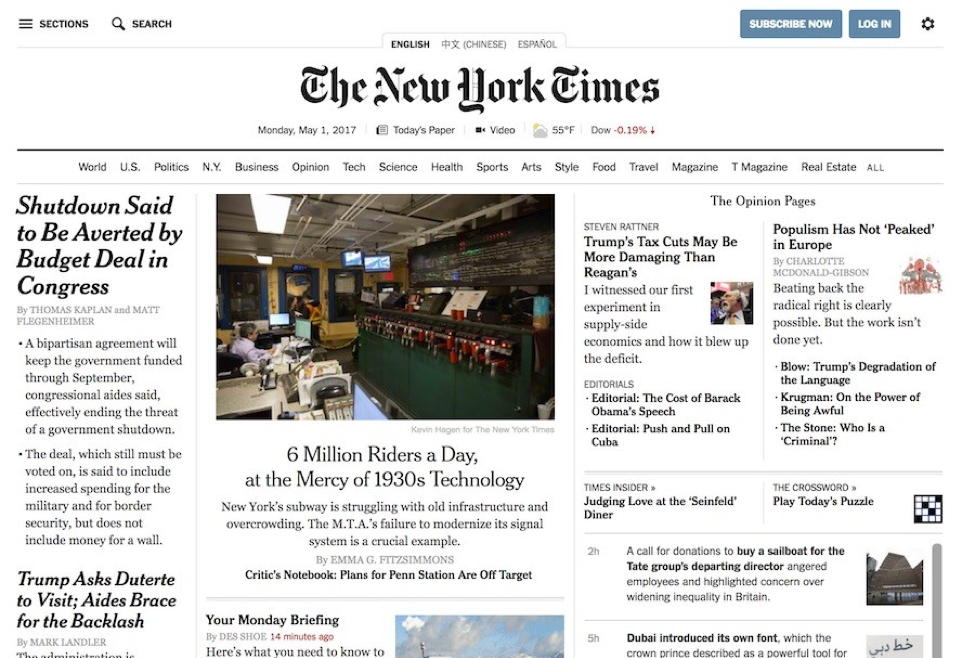
\includegraphics[scale=0.8]{Figures/pic16.png}
    \caption{NewYork times хуудас}
    \label{fig16}
\end{figure}\\
\begin{itemize}
    \item [\textbf{5.}] \textbf{Yahoo! Мэйл}
\end{itemize}
Yahoo!-ийн мэйл клиент нь мөн React ашигладаг. Facebook нь Yahoo! Өнөө үед хатуу, нэгдмэл архитектурын санаа байдаг бөгөөд иймээс React-ийг аль болох олон хэсэг болгон нэгтгэсэн. React-ээр тусгайлан бүтээгдсэн архитектурыг эндээс харж болно – мөн Yahoo! Хөгжүүлэгчид үүнийг кодтой ажиллахад илүү хялбар, илүү сайн гэж дүгнэж байна.
\begin{itemize}
    \item [\textbf{6.}] \textbf{Khan Academy}
\end{itemize}
Хан Академийн ихэнх хэсэг нь одоогоор React дээр суурилсан. Тэдний JavaScript хөгжүүлэгчдийн нэг Жоэл Бургет ReactJS номын сантай холбоотой туршлагаасаа хуваалцаж, энэ нь тэдний өмнө нь ашиглаж байсан уламжлалт Backbone скриптээс хэрхэн ялгагдах талаар хуваалцав.Тэрээр үүнийг зохистой шинэчлэл гэж тодорхойлж, элементийг үр ашигтайгаар өөрчлөх, шаардлагагүй дахин дүрслэлийг арилгах зэрэг ихэнх чухал шинж чанаруудыг анхааралтай судалж үздэг.
\begin{itemize}
    \item [\textbf{7.}] \textbf{WhatsApp}
\end{itemize}
Хэдийгээр албан ёсоор нээлтээ хийхээс өмнө хэд хэдэн бета хувилбарууд байсан ч WhatsApp нь Underscore.js болон Velocity.js-ийг хамгийн үр ашигтай хөдөлгүүр болгон ашигладагтай адил Facebook-ээс хэрэглэгчийн интерфэйс бүтээхэд ReactJS ашигладаг.
\begin{itemize}
    \item [\textbf{8.}] \textbf{Vivaldi хөтөч}
\end{itemize}
Алдартай Vivaldi Browser-ийн ард байгаа технологийн нэг бол ReactJS номын сан юм. Энэхүү хөтчийн ашиглаж буй хөдөлгүүр нь 'Blink' нэртэй бөгөөд HTML5, ReactJS, JS, CSS3 болон бусад олон хөдөлгүүр дээр бүтээгдсэн Google-ийн Chrome-той бараг адилхан юм.
\begin{itemize}
    \item [\textbf{9.}] \textbf{Codecademy}
\end{itemize}
2014 оны 8-р сарын байдлаар Codecademy нь Facebook-ийн номын санг бүрэн хэмжээгээр оруулахаар шийдсэн. ReactJS нь мэдээжийн хэрэг түүний нэг хэсэг байсан бөгөөд одоо ч програм дээр суурилсан гол скриптүүдийн нэг хэвээр байна.Гарчигнаас эхлээд цэс, тэр ч байтугай навигац хүртэл ReactJS хэрэглээ нь Codeacademy дээр байдаг бөгөөд янз бүрийн хэсгүүдэд зориулсан бүх бүрэлдэхүүн хэсгүүдийг багтаасан логик шийдэл болгон бүтээгдсэн. Codeacademy-ийн бүх хүмүүсийн үзэж байгаагаар React-ийн зарим тал нь тэдний талархаж буй скрипт нь тулалдаанд туршиж үзсэн, бодоход хялбар, SEO-г хялбар болгодог, хуучин кодтой нийцэж, ирээдүйд хангалттай уян хатан байдаг. Түүнчлэн, энэ нь олон нийтийг бий болгоход түлхэц өгч, уурын зуухны талаар санаа зовохоо болих боломжийг танд олгоно.
\begin{itemize}
    \item [\textbf{10.}] \textbf{Dropbox}
\end{itemize}
Dropbox жил гаруйн өмнө ReactJS рүү шилжсэн. Яг тэр үед React програм хөгжүүлэгчдийн дунд маш их алдартай болсон. Энэхүү тогтолцооны нэг хэсэг болох олон нөөцийг Dropbox үр ашигтай ашигладаг бөгөөд энэ нь үүлэнд суурилсан хадгалалтын үйлчилгээ болон онлайн нөөцлөлтийн шийдлийн амжилтанд ихээхэн хувь нэмэр оруулдаг.
\begin{table}[ht]
    \centering
    \begin{tabular}{|p{2cm}|p{5cm}|p{7cm}|}
         \hline
         Хэл &	Хэрэглээ &	Онцлог шинжүүд \\ \hline
         HTML &	Вeб хуудасны бүтэц, агуулга & Гарчиг, догол мөр, зураг, холбоос, маягт зэрэг элементүүдийг тодорхойлдог \\ \hline
         CSS & Вeб хуудасны загвар, танилцуулга & Өнгө, фонт, байршил, хөдөлгөөнт дүрс зэрэг функцээр гадаад төрхийг хянадаг\\ \hline
         JavaScript & Вeб хуудсанд интерактив нэмэх & Маягтыг баталгаажуулах, DOM удирдах, үйл явдлыг зохицуулах, сервертэй харилцах зэрэг ажлуудыг идэвхжүүлдэг\\ \hline
         React & Хэрэглэгчийн интерфейсийг бий болгох JavaScript номын сан & Бүрэлдэхүүн хэсгүүдэд суурилсан архитектурыг дагаж, дахин ашиглах боломжтой UI бүрэлдэхүүн хэсгүүдийг бий болгох боломжийг олгодог \\ \hline
    \end{tabular}
    \caption{Вэб хэлний харьцуулалт}
    \label{tab11}
\end{table}\\
\newpage
\section{Өгөгдлийн сан гэж юу вэ?}
Өгөгдлийн сан (Database) нь тодорхой зорилгоор хамтад нь цуглуулж, тодорхой зохион байгуулалттайгаар компьютерын тогтмол санах ойд хадгалсан цогц өгөгдлийн цуглуулга. Өгөгдлийн сантай бүхий л хэлбэрээр ажиллахад зориулсан компьютерын программ хангамжийг DBMS (Database Management System) буюу ӨСУС (Өгөгдлийн санг удирдах систем) гэнэ. Үүнийг ашиглаад хэрэглэгч нь өгөгдлийн сантай харилцах бөгөөд эмх цэгцтэйгээр хадгалах, богино хугацаанд хайх, нууцлал хамгаалалтыг сайжруулах гэх мэт төрөл бүрийн зүйлсийг автоматаар шийдэж өгсөн байдаг. Маш олон нэр төрлийн ӨСУС-ууд байдгаас жишээ татвал: MySQL, MSSQL, PostgreSQL, MongoDB, Cassandra, SQLite г.м. 
\begin{figure}[hb]
    \centering
    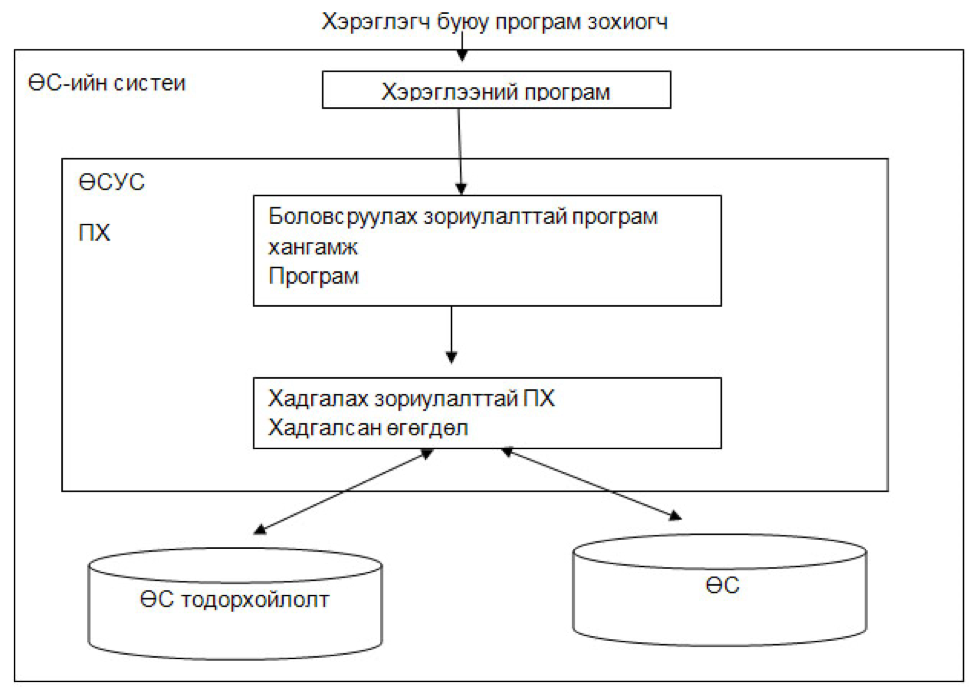
\includegraphics[scale=0.7]{Figures/pic17.png}
    \caption{Өгөгдлийн санг удирдах систем}
    \label{fig17}
\end{figure}\\
Өгөгдлийн сангийн олон төрөл байдаг. Тухайн байгууллагын хамгийн сайн мэдээллийн сан нь тухайн байгууллага тухайн өгөгдлийг хэрхэн ашиглахаар төлөвлөж байгаагаас хамаарна.
\begin{itemize}
    \item [•] \textbf{Харилцааны мэдээллийн сан (Relational databases)}
\end{itemize}
1980-аад онд харилцааны мэдээллийн сан давамгайлах болсон. Харьцааны мэдээллийн сан дахь зүйлсийг багана, мөр бүхий хүснэгтүүдийн багц хэлбэрээр зохион байгуулдаг. Харилцааны мэдээллийн сангийн технологи нь бүтэцлэгдсэн мэдээлэлд хандах хамгийн үр дүнтэй, уян хатан аргыг олгодог.
\begin{itemize}
    \item [•] \textbf{Объект хандалтат мэдээллийн сан (Object-oriented databases)}
\end{itemize}
Объект хандалтат өгөгдлийн сан дахь мэдээлэл нь объект хандалтат програмчлалын нэгэн адил объект хэлбэрээр илэрхийлэгддэг.
\begin{itemize}
    \item [•] \textbf{Түгээмэл мэдээллийн сан (Distributed databases)}
\end{itemize}
Түгээмэл мэдээллийн сан нь өөр өөр сайтуудад байрлах хоёр ба түүнээс дээш файлуудаас бүрддэг. Өгөгдлийн сан нь нэг физик байршилд байрлах, эсвэл өөр өөр сүлжээгээр тархсан олон компьютер дээр хадгалагдаж болно.
\begin{itemize}
    \item [•] \textbf{Мэдээллийн агуулахууд (Data warehouses)}
\end{itemize}
Мэдээллийн төвлөрсөн агуулах, мэдээллийн агуулах нь хурдан хайлт хийх, дүн шинжилгээ хийхэд зориулагдсан мэдээллийн сангийн төрөл юм.
\begin{itemize}
    \item [•] \textbf{NoSQL мэдээллийн сан (NoSQL databases)}
\end{itemize}
NoSQL буюу хамааралгүй өгөгдлийн сан нь бүтэцгүй болон хагас бүтэцтэй өгөгдлийг хадгалах, удирдах боломжийг олгодог (өгөгдлийн санд оруулсан бүх өгөгдөл хэрхэн бүрдэх ёстойг тодорхойлдог харилцааны мэдээллийн сангаас ялгаатай). 
\begin{itemize}
    \item [•] \textbf{График мэдээллийн сан (Graph databases)}
\end{itemize}
\begin{itemize}
    \item [1.] График мэдээллийн сан нь өгөгдлийг аж ахуйн нэгжүүд болон аж ахуйн нэгжүүдийн хоорондын харилцааны хувьд хадгалдаг.
    \item [2.] OLTP мэдээллийн сан. OLTP мэдээллийн сан нь олон хэрэглэгчийн гүйцэтгэсэн олон тооны гүйлгээнд зориулагдсан хурдан, аналитик мэдээллийн сан юм.
\end{itemize}
Эдгээр нь өнөөдөр ашиглагдаж буй хэдэн арван төрлийн мэдээллийн сангаас хэдхэн нь юм. Бусад бага түгээмэл мэдээллийн сангууд нь шинжлэх ухаан, санхүүгийн болон бусад чиг үүрэгт тохирсон байдаг. Мэдээллийн сангийн янз бүрийн төрлөөс гадна технологийн хөгжлийн арга барилд гарсан өөрчлөлт, үүлэн систем, автоматжуулалт зэрэг гайхалтай дэвшил нь мэдээллийн санг цоо шинэ чиглэлд түлхэж байна.
\begin{itemize}
    \item [•] \textbf{Нээлттэй эхийн мэдээллийн сан (Open source databases)}
\end{itemize}
Нээлттэй эхийн өгөгдлийн сангийн систем нь эх код нь нээлттэй эхийн систем юм. Ийм мэдээллийн сан нь SQL эсвэл NoSQL мэдээллийн сан байж болно.
\begin{itemize}
    \item [•] \textbf{Үүлэн мэдээллийн сан (Cloud databases)}
\end{itemize}
Үүлэн мэдээллийн сан нь хувийн, нийтийн эсвэл эрлийз үүлэн тооцооллын платформ дээр байрладаг бүтэцтэй эсвэл бүтэцгүй мэдээллийн цуглуулга юм. Уламжлалт ба өгөгдлийн сангийн үйлчилгээ (DBaaS) гэсэн хоёр төрлийн үүлэн мэдээллийн сан загвар байдаг. DBaaS-ийн тусламжтайгаар захиргааны ажил, засвар үйлчилгээг үйлчилгээ үзүүлэгч гүйцэтгэдэг.
\begin{itemize}
    \item [•] \textbf{Олон загварын мэдээллийн сан (Multimodel database)}
\end{itemize}
Multimodel database нь янз бүрийн төрлийн мэдээллийн баазын загваруудыг нэг, нэгдсэн арын төгсгөлд нэгтгэдэг. Энэ нь тэд янз бүрийн өгөгдлийн төрлийг багтааж чадна гэсэн үг юм.
\begin{itemize}
    \item [•] \textbf{Баримт бичиг/JSON мэдээллийн сан (Document/JSON database)}
\end{itemize}
Баримт бичигт чиглэсэн мэдээллийг хадгалах, сэргээх, удирдахад зориулагдсан баримт бичгийн мэдээллийн сан нь мөр, багана гэхээсээ илүү JSON форматаар өгөгдлийг хадгалах орчин үеийн арга юм.
\begin{itemize}
    \item [•] \textbf{Өөрөө жолооддог мэдээллийн сан (Self-driving databases)}
\end{itemize}
Өгөгдлийн сангийн шинэ бөгөөд шинэлэг төрөл болох өөрөө жолооддог мэдээллийн сан (өөрийгөө бие даасан мэдээллийн сан гэж нэрлэдэг) нь үүлд суурилсан бөгөөд мэдээллийн сангийн тохируулга, аюулгүй байдал, нөөцлөлт, шинэчлэлт болон бусад ердийн удирдлагын даалгавруудыг автоматжуулахын тулд өгөгдлийн сангийн администраторуудыг уламжлалт байдлаар гүйцэтгэдэг.\\
Өгөгдлийн сангийн бүрэлдэхүүн хэсгүүд:\\
Өгөгдлийн сангийн янз бүрийн төрлүүд нь схем, өгөгдлийн бүтэц, өгөгдлийн төрлөөрөө өөр өөр байдаг ч тэдгээр нь бүгд ижил таван үндсэн бүрэлдэхүүн хэсгээс бүрддэг.
\begin{itemize}
    \item [1.] \textbf{Техник хангамж.} Энэ бол мэдээллийн сангийн програм хангамж дээр ажилладаг физик төхөөрөмж юм. Өгөгдлийн сангийн техник хангамжид компьютер, сервер, хатуу диск орно.
    \item [2.] \textbf{Програм хангамж.} Өгөгдлийн сангийн програм хангамж эсвэл програм нь хэрэглэгчдэд мэдээллийн баазыг хянах боломжийг олгодог. Өгөгдлийн сангийн удирдлагын систем (DBMS) программ хангамжийг мэдээллийн санг удирдах, хянахад ашигладаг.
    \item [3.] \textbf{Өгөгдөл.} Энэ бол мэдээллийн санд хадгалагдаж буй түүхий мэдээлэл юм. Өгөгдлийг илүү утга учиртай болгох үүднээс зохион байгуулдаг.
    \item [4.] \textbf{Өгөгдөл хандалтын хэл.} Энэ бол мэдээллийн санг хянадаг програмчлалын хэл юм. Програмчлалын хэл болон DBMS нь хамтран ажиллах ёстой. Өгөгдлийн сангийн хамгийн түгээмэл хэлнүүдийн нэг бол SQL юм.
    \item [5.] \textbf{Процедурууд.} Эдгээр дүрмүүд нь мэдээллийн сан хэрхэн ажилладаг, өгөгдөлтэй хэрхэн харьцдагийг тодорхойлдог.
\end{itemize}
\begin{figure}[ht]
    \centering
    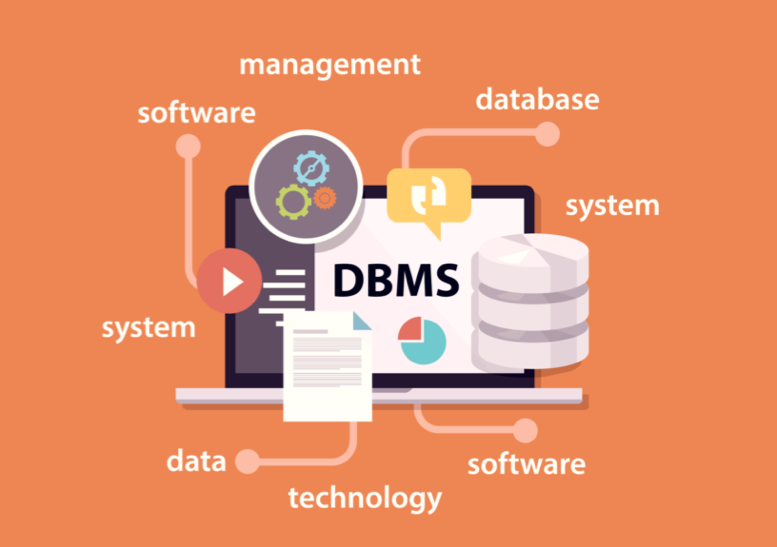
\includegraphics[scale=0.8]{Figures/pic18.png}
    \caption{Өгөгдлийн сангийн удирдлагын систем}
    \label{fig18}
\end{figure}
Өгөгдлийн сан нь ихэвчлэн мэдээллийн сангийн удирдлагын систем (DBMS) гэгддэг мэдээллийн сангийн иж бүрэн програм хангамжийг шаарддаг. DBMS нь өгөгдлийн сан болон түүний эцсийн хэрэглэгчид эсвэл программуудын хооронд интерфэйс болж, хэрэглэгчдэд мэдээллийг хэрхэн зохион байгуулж, оновчтой болгохыг сэргээх, шинэчлэх, удирдах боломжийг олгодог. Мөн DBMS нь мэдээллийн сангийн хяналт, хяналтыг хөнгөвчлөх бөгөөд гүйцэтгэлийг хянах, тохируулах, нөөцлөх, сэргээх зэрэг олон төрлийн захиргааны үйл ажиллагааг идэвхжүүлдэг.\\
Алдартай мэдээллийн сангийн програм хангамж эсвэл DBMS-ийн зарим жишээнд MySQL, Microsoft Access, Microsoft SQL Server, FileMaker Pro, Oracle Database, dBASE орно.\\
\textbf{Өгөгдлийн сангуудын харьцууллалт}
\begin{table}[ht]
    \centering
    \begin{tabular}{|p{3cm}|p{7cm}|p{3cm}|}
    \hline
    Өгөгдлийн сангийн төрөл &	Тайлбар &	Жишээ \\ \hline
    Relational & Урьдчилан тодорхойлсон схемүүд болон хүснэгтүүдийн хоорондын хамаарал бүхий хүснэгтүүдийг зохион байгуулдаг. & MySQL, PostgreSQL, Oracle \\ \hline
    NoSQL & Өгөгдлийг янз бүрийн форматаар (түлхүүр утга, баримт бичиг, багана, график) хадгалдаг уян хатан, схемгүй мэдээллийн сан. & MongoDB, Cassandra, Redis \\ \hline
    NewSQL & Relational болон NoSQL өгөгдлийн сангийн ашиг тусыг нэгтгэх, өргөтгөх чадвар, өндөр гүйцэтгэлийг хангах зорилготой мэдээллийн сангийн шинэ анги. & CockroachDB, Google Spanner, TiDB\\ \hline
    Graph & Өгөгдлийг зангилаа болон харилцаа хэлбэрээр илэрхийлэх, хадгалахад зориулагдсан бөгөөд нарийн төвөгтэй харилцааг туулахад оновчтой болгосон. & Neo4j, Amazon Neptune, JanusGraph \\ \hline
    Time Series & IoT мэдрэгчийн уншилт эсвэл санхүүгийн зах зээлийн мэдээлэл гэх мэт цаг хугацааны тамгатай их хэмжээний өгөгдлийг боловсруулахад оновчтой. & InfluxDB, Prometheus, TimescaleDB\\ \hline
    In-Memory & Өгөгдөл нь үндсэндээ санах ойд хадгалагддаг тул өгөгдөлд хандах, боловсруулах хурд илүү хурдан болдог. & Redis, Memcached, Apache Ignite \\ \hline
    Columnar & Мэдээллийг мөр биш баганад хадгалснаар тодорхой өгөгдлийн дэд бүлгүүдийг үр ашигтай хадгалах, сэргээх боломжийг олгодог. & Apache Cassandra, Amazon Redshift\\ \hline
    Document & Хагас бүтэцтэй эсвэл бүтэцгүй өгөгдлийг JSON шиг уян хатан баримт бичигт хадгалдаг. & MongoDB, CouchDB, Elasticsearch\\ \hline
    \end{tabular}
    \caption{Өгөгдлийн сангийн харьцуулалт}
    \label{tab12}
\end{table}
\section{MongoDB гэж юу вэ?}
MongoDB нь уян хатан, өргөтгөх боломжтой, ашиглахад хялбар гэдгээрээ алдартай, нээлттэй эхийн NoSQL мэдээллийн сан юм. Энэ нь NoSQL- д хамаарах баримт бичигт чиглэсэн мэдээллийн сан бөгөөд энэ нь уламжлалт харилцааны өгөгдлийн сангийн загварт тулгуурладаггүй гэсэн үг юм.\\
MongoDB нь өгөгдлийг BSON (Binary JSON) хэмээх уян хатан, JSON-той төстэй баримт бичигт хадгалдаг бөгөөд энэ нь нарийн төвөгтэй өгөгдлийн бүтцийг дүрслэх боломжийг олгодог. Эдгээр баримт бичиг нь бүтцийн хувьд өөр байж болох тул MongoDB нь хагас бүтэцтэй болон бүтэцгүй өгөгдөлтэй ажиллахад маш тохиромжтой.\\
MongoDB-ийн гол онцлогууд нь:
\begin{itemize}
    \item [1.] Баримт бичигт чиглэсэн: Өгөгдөл нь уян хатан, өөрөө тайлбарлах боломжтой баримт бичигт хадгалагдаж, схемийг хялбар, динамик өөрчлөх боломжийг олгодог.
    \item [2.] Өргөтгөх чадвар: MongoDB нь олон серверт хэвтээ байдлаар масштаблах боломжтой бөгөөд ачаалал ихтэй, том өгөгдлийн багцыг зохицуулахын тулд кластерт өгөгдөл болон ачааллыг түгээх боломжтой.
    \item [3.] Өндөр гүйцэтгэл: MongoDB нь дотоод санах ойг ажлын багц хадгалахад ашигладаг бөгөөд ингэснээр унших, бичих үйлдлийг хурдан гүйцэтгэдэг. Энэ нь мөн үр дүнтэй асуулга хийх индексүүдийг дэмждэг.
    \item [4.] Асуулга ба нэгтгэх: MongoDB нь шүүлтүүр, эрэмбэлэх, нэгдэх зэрэг өргөн хүрээний асуулгад зориулсан хүчирхэг хайлтын хэлээр хангадаг. Энэ нь мэдээллийн дэвшилтэт боловсруулалт, дүн шинжилгээ хийхэд зориулж нэгтгэх дамжуулах шугамыг дэмждэг.
    \item [5.] Хуулбарлах ба алдааг тэсвэрлэх чадвар: MongoDB нь өгөгдлийг автоматаар хуулбарлахыг дэмждэг бөгөөд энэ нь өндөр хүртээмжтэй, алдааг тэсвэрлэх боломжийг олгодог. Энэ нь серверийн доголдол гарсан тохиолдолд өгөгдлийн бат бөх байдал, сэргэлтийг баталгаажуулдаг.
    \item [6.] Гео орон зайн боломжууд: MongoDB нь гео орон зайн индекс, асуулга агуулсан бөгөөд газарзүйн өгөгдлийг хадгалах, сэргээх, ойрын зайд суурилсан хайлт хийх боломжийг олгодог.
\end{itemize}
MongoDB нь агуулгын удирдлагын систем, цахим худалдааны платформ, бодит цагийн аналитик, өгөгдөл их шаарддаг программ зэрэг төрөл бүрийн хэрэглээнд өргөн хэрэглэгддэг. Түүний уян хатан шинж чанар, хэвтээ өргөтгөх боломжтой, баялаг боломжууд нь олон талт, өргөтгөх боломжтой мэдээллийн сангийн шийдлийг эрэлхийлдэг хөгжүүлэгчдэд түгээмэл сонголт болгодог.\\
\textbf{MongoDB хэрхэн ажилладаг вэ?}\\
MongoDB орчин нь хэрэглэгчдэд MongoDB-тэй мэдээллийн сан үүсгэх серверээр хангадаг. MongoDB нь өгөгдлийг цуглуулга, баримт бичгээс бүрдсэн бичлэг болгон хадгалдаг.\\
Баримт бичиг нь хэрэглэгчийн MongoDB мэдээллийн санд хадгалахыг хүссэн өгөгдлийг агуулна. Баримт бичгүүд нь талбар ба утгын хосуудаас бүрдэнэ. Эдгээр нь MongoDB дахь өгөгдлийн үндсэн нэгж юм. Баримт бичгүүд нь JavaScript Object Notation (JSON)-тай төстэй боловч Binary JSON (BSON) нэртэй хувилбарыг ашигладаг. BSON ашиглахын давуу тал нь илүү олон өгөгдлийн төрлийг багтаах явдал юм. Эдгээр баримт бичгийн талбарууд нь харилцааны мэдээллийн сангийн баганатай адил юм. MongoDB хэрэглэгчийн гарын авлагын дагуу бусад баримт бичиг, массив, баримт бичгийн массив зэрэг олон төрлийн өгөгдлийн төрлүүд байж болно. Мөн баримт бичигт үндсэн түлхүүрийг өвөрмөц танигч болгон агуулна. Баримт бичгийн бүтцийг шинэ эсвэл одоо байгаа талбаруудыг нэмэх, устгах замаар өөрчилдөг.\\
Mongo shell нь MongoDB-ийн нээлттэй эхийн түгээлтийн стандарт бүрэлдэхүүн хэсэг юм. MongoDB суулгасны дараа хэрэглэгчид mongo shell-ийг ажиллаж байгаа MongoDB instance-тэй холбодог. Mongo shell нь MongoDB-ийн интерактив JavaScript интерфэйсийн үүрэг гүйцэтгэдэг бөгөөд энэ нь хэрэглэгчдэд өгөгдөл асуух, шинэчлэх, удирдлагын үйл ажиллагаа явуулах боломжийг олгодог.\\
JSON-тэй төстэй баримт бичгийн хоёртын дүрслэлийг BSON баримт хадгалах болон өгөгдөл солилцох форматаар хангадаг. Автомат хуваах нь өгөгдлийн хэмжээ болон дамжуулах чадварын шаардлага нэмэгдэхийн хэрээр MongoDB цуглуулгад байгаа өгөгдлийг хэвтээ байдлаар өргөтгөх зорилгоор олон системд түгээх боломжийг олгодог нь нэг гол онцлог юм.\\
\textbf{MongoDB-ийн давуу тал}
\begin{itemize}
    \item [•] Схемгүй. Бусад NoSQL мэдээллийн сангийн нэгэн адил MongoDB нь урьдчилан тодорхойлсон схемүүдийг шаарддаггүй. Энэ нь ямар ч төрлийн өгөгдлийг хадгалдаг. Энэ нь хэрэглэгчдэд баримт бичигт хэдэн ч талбар үүсгэх уян хатан боломжийг олгож, MongoDB мэдээллийн санг харилцааны өгөгдлийн сантай харьцуулахад илүү хялбар болгодог.
    \item [•] Баримт бичигт чиглэсэн. Баримт бичгийг ашиглахын нэг давуу тал нь эдгээр объектууд нь хэд хэдэн програмчлалын хэл дээрх эх өгөгдлийн төрлүүдтэй зураглагддаг явдал юм. Мөн суулгагдсан баримтууд нь мэдээллийн санд нэгдэх хэрэгцээг багасгаж, зардлыг бууруулж чадна.
    \item [•] Өргөтгөх чадвар. MongoDB-ийн үндсэн үүрэг бол хэвтээ өргөтгөх чадвар бөгөөд энэ нь том дата програм ажиллуулдаг компаниудад хэрэгтэй мэдээллийн сан болгодог. Нэмж дурдахад, sharding нь мэдээллийн санд өгөгдлийг кластерийн машинуудад түгээх боломжийг олгодог. Мөн MongoDB нь хэлтэрхий түлхүүр дээр тулгуурлан өгөгдлийн бүс үүсгэхийг дэмждэг.
    \item [•] Гуравдагч талын дэмжлэг. MongoDB нь хэд хэдэн хадгалах системийг дэмждэг бөгөөд залгагддаг санах ойн хөдөлгүүрийн API-уудыг хангадаг бөгөөд энэ нь гуравдагч этгээдэд MongoDB-д зориулж өөрсдийн хадгалах системийг хөгжүүлэх боломжийг олгодог.
    \item [•] Нэгтгэх. Мөн DBMS нь нэгтгэсэн нэгтгэх чадвартай бөгөөд энэ нь хэрэглэгчдэд MapReduce кодыг Hadoop дээр ажиллуулахын оронд шууд мэдээллийн сан дээр ажиллуулах боломжийг олгодог. MongoDB нь Hadoop Distributed File System-тэй адил GridFS нэртэй өөрийн файлын системийг агуулдаг. Файлын системийг ашиглах нь үндсэндээ BSON-ын хэмжээ хязгаараас нэг баримт бичигт 16 МБ-аас их хэмжээтэй файлуудыг хадгалахад зориулагдсан. Эдгээр ижил төстэй байдал нь MongoDB-г Hadoop-ийн оронд ашиглах боломжийг олгодог боловч мэдээллийн сангийн програм хангамж нь Hadoop, Spark болон бусад өгөгдөл боловсруулах хүрээтэй нэгтгэдэг.
\end{itemize}
\textbf{MongoDB-ийн сул тал}
\begin{itemize}
    \item [•] Тасралтгүй байдал. Автомат шилжүүлгийн стратегийн тусламжтайгаар хэрэглэгч MongoDB кластерт зөвхөн нэг мастер зангилааг тохируулдаг. Хэрэв мастер амжилтгүй болвол өөр зангилаа автоматаар шинэ мастер руу хөрвүүлнэ. Энэ шилжүүлэгч нь тасралтгүй байдлыг амлаж байгаа ч энэ нь шууд биш, нэг минут хүртэл хугацаа шаардагдах болно. Харьцуулбал, Кассандра NoSQL мэдээллийн сан нь олон мастер зангилааг дэмждэг. Хэрэв нэг мастер унтарвал нөгөө мастер нь зогсож, өндөр хүртээмжтэй мэдээллийн сангийн дэд бүтцийг бий болгодог.
    \item [•] Хязгаарыг бичих. MongoDB-ийн нэг мастер зангилаа нь өгөгдлийн санд өгөгдлийг хэр хурдан бичихийг хязгаарладаг. Өгөгдлийн бичгийг мастер дээр бичих ёстой бөгөөд мэдээллийн санд шинэ мэдээлэл бичих нь тухайн мастер зангилааны хүчин чадлаар хязгаарлагддаг.
    \item [•] Өгөгдлийн тууштай байдал. MongoDB нь гадаад түлхүүрийн хязгаарлалтыг ашиглан лавлагааны бүрэн бүтэн байдлыг хангадаггүй бөгөөд энэ нь өгөгдлийн тогтвортой байдалд нөлөөлж болзошгүй.
    \item [•] Аюулгүй байдал. Нэмж дурдахад, MongoDB мэдээллийн санд хэрэглэгчийн баталгаажуулалтыг анхдагчаар идэвхжүүлээгүй байна. Гэсэн хэдий ч хорлонтой хакерууд халдлагад олон тооны хамгаалалтгүй MongoDB системүүдийг онилсон бөгөөд энэ нь мэдээллийн сангийн администратороор тохируулаагүй тохиолдолд мэдээллийн санд холбогдох сүлжээний холболтыг хаадаг анхдагч тохиргоог нэмэхэд хүргэсэн.
\end{itemize}
\textbf{MongoDB ба RDBMS: Ялгаа нь юу вэ?}\\
Харилцааны мэдээллийн баазын удирдлагын систем (RDBMS) нь мэдээллийн технологийн баг болон бусад хүмүүст харилцааны мэдээллийн санг үүсгэх, шинэчлэх, удирдах болон бусад аргаар харилцах боломжийг олгодог программууд болон чадавхуудын цуглуулга юм. RDBMS нь өгөгдлийг хүснэгт, мөр хэлбэрээр хадгалдаг. Энэ нь шаардлагагүй ч RDBMS нь SQL-г ихэвчлэн ашигладаг.\\
MongoDB болон RDBMS-ийн гол ялгааны нэг нь RDBMS нь харилцааны мэдээллийн сан, харин MongoDB нь хамааралгүй байдаг. Үүний нэгэн адил ихэнх RDBMS системүүд хадгалагдсан өгөгдлийг удирдахын тулд SQL ашигладаг бол MongoDB нь NoSQL мэдээллийн сангийн төрөл болох өгөгдөл хадгалахад BSON ашигладаг.\\
RDBMS нь хүснэгт, мөрүүдийг ашигладаг бол MongoDB нь баримт бичиг, цуглуулгуудыг ашигладаг. RDBMS-д MongoDB цуглуулгатай тэнцэх хүснэгт нь өгөгдлийг багана, мөр хэлбэрээр хадгалдаг. Үүний нэгэн адил RDBMS дахь мөр нь MongoDB баримт бичигтэй тэнцэх боловч өгөгдлийг хүснэгтэд бүтэцлэгдсэн өгөгдлийн зүйл болгон хадгалдаг. Багана нь өгөгдлийн утгуудын багцыг илэрхийлдэг бөгөөд энэ нь MongoDB дахь талбартай тэнцүү юм.\\
\textbf{MongoDB платформууд}\\
MongoDB нь олон нийтийн болон арилжааны хувилбаруудыг борлуулагч MongoDB Inc-ээр дамжуулан авах боломжтой. MongoDB Community Edition нь нээлттэй эхийн хувилбар бөгөөд MongoDB Enterprise Server нь нэмэлт хамгаалалтын функцууд, санах ойн санах ойн систем, удирдлага болон баталгаажуулалтын функцууд болон Ops Manager-ээр дамжуулан хяналтын боломжуудыг авчирдаг.\\
MongoDB Compass нэртэй график хэрэглэгчийн интерфэйс (GUI) нь хэрэглэгчдэд баримт бичгийн бүтэцтэй ажиллах, асуулга явуулах, индексийн өгөгдөл болон бусад зүйлсийг хийх боломжийг олгодог. BI-д зориулсан MongoDB холбогч нь хэрэглэгчдэд SQL асуулга ашиглан өгөгдлийг дүрслэн харуулах, тайлан үүсгэхийн тулд NoSQL мэдээллийн баазыг бизнесийн тагнуулын хэрэгслүүдтэй холбох боломжийг олгодог.